\documentclass[11pt]{article}
\usepackage[utf8]{inputenc}
\usepackage[margin=1.3in]{geometry}
\usepackage[hidelinks]{hyperref}
%\usepackage{eurosym}
\usepackage{caption}
\usepackage{titling}
\usepackage{xcolor,colortbl}
\usepackage{tabularx}
\usepackage{changepage}
\usepackage{multicol}
\usepackage{graphicx}
\graphicspath{ {./img/} }
%------------------------------------------
\captionsetup[table]{position=bottom}
\setlength{\parindent}{0pt}
\definecolor{Gray}{rgb}{0.7,0.7,0.7}
\pretitle{\begin{center}\Large\bfseries}
%------------------------------------------



\title{
  Serverless technologies comparison\\
  \large Large Systems project}
\author{Sean Liao and Mar Badias}



\begin{document}

\maketitle

%% TODO abstract
%% TODO introduction
  %% -> why our reaserch is relevant, what are this services exactly
  %% -> why can we put Caas and FaaS in the same bag

%% TODO related work
%% TODO research question
%% - business case/
%% TODO methodology
%% - variables
%% - CPU
%% - overhead / latencies
%% - pricing model
%% - test setup
%% TODO results
%% - data
%% - pricing
%% TODO discussion
%% - applicability
%% - billing
%% - other tech
%% - answer reaserch question
%% TODO usage case
%% TODO future work
%% TODO conclusion
%% TODO references

%coses q haurien de quedar molt clares: cold starts



\begin{abstract}
Write abstrat here
\end{abstract}

\newpage

\section{Introduction}
\label{introduction}

% todo: narrow title scope
% todo: define PaaS, FaaS, CaaS, cold start
% todo: introduce common usecase: why people choose serverless
% skip selection

Public clouds are growing, and with it comes the latest push into serverless offerings. These come in many forms depending on the abstraction level, but they can largely be grouped into: long-lived containers, short-lived containers, functions as a service. \\

Long-lived containers or Platform as a Service (PaaS) represent the first generation of serverless technologies. These can be full-fledged, stateful applications, packaged in containers. The clouds will take these and run them for you on VMs. Auto-scaling and load balancing is usually offered, but fast startup times are not guaranteed. These should be considered an alternative UI to the underlying VMs, which will be reflected in the pricing model (charge for underlying VMs). Examples: AWS Elastic Container service, GCP App Engine, Azure App Services, Alibaba Container Service. \\

Functions as a Service (FaaS), currently the highest level of abstraction and the second generation of serverless technologies. Developers provide their application code for the clouds to compile, package, deploy, and run. These are short-lived and stateless, an instance may be started for every request and killed after it completes. Billing is only for the time it is running serving a request. Examples: AWS Lambda, GCP Cloud Functions, Azure Functions, Alibaba Function Compute, IBM Cloud Functions, Zeit Now.\\

Short-lived containers or Containers as a Service (CaaS). Is the newest technologies short-lived, stateless runtimes and a similar billing model. Where they differ from FaaS is that they introduce containers, giving developers control of the execution environment, allowing them to run languages or runtimes unsupported by FaaS. Examples: AWS Fargate, GCP Cloud Run, Azure Container Instance, Alibaba Elastic Container Instance. \\


insert why people use serverless. \\

Our reaserch will measure and analiyse its CPU performance, overhead and specially their capacity to scale when the workload increases. Scaling entails creating more instances, known as cold starts, and assigning new resources between them without influencing others' instances performance.


\section{Related work}

Serverless technologies have been subject of previous research.
We can find good examples of PaaS analysis in \cite{googleappengine} and \cite{googleappengine2},
where the reaserchers analize Google App Enginee performance with CPU-intensive applications.
CaaS have also been a topic of study,
comparing them to long live containers or performance test among of different provides.
We can find examples of this in \cite{cc} and \cite{dd}.
Comparison between Faas and short-lived containers has also been analized
but from a functionality point of view
but oversimplificating it and not taking into account the performance \cite{ee}\cite{ff}\cite{gg}. \\

FaaS on its own also has been subject of previous research.
An excellent example is \cite{aa}
where multiple serverless providers are continuously been benchmarked.
Another example of a comparison of Faas providers is \cite{bb}.
In \cite{14} the researches dicuss the advantages of using cloud services
and AWS Lambada for systems that require higher resilance.
Finally, is necessary to mention \cite{https://sci-hub.se/10.1002/cpe.4792},
which fouses in its performance evaluation
and also benchmarking the data transfer to storage and its lifetime of the major cloud functions providers. \\

Aldought serverless performance has been heavily analized,
to the best of our knowledge their scaling and its consequences to performance
and overhead have not been comprehensively analysed yet, which motivates our research.


\section{Research question}

\begin{itemize}
\item \textbf{How do different platforms compare when with sudden spikes in traffic?}
\end{itemize}

Specifically we will be looking at:

\begin{itemize}

\item \textbf{Does scaling out affect the performance of the services?}
When scaling out to meet demand,
serverless platforms should isolate instances
to provide a consistent level of performance.

\item \textbf{Does scaling out affect platform overhead}
Everything has a cost,
what we hope to see is that scaling out does not severely degrade the platform's performance,
in terms of instance management.
\end{itemize}


\section{Methods}
\label{methods}

Given the amount of services of this type in the current market we defined a selection criteria based on the most popular features \cite{popular1} of serverless computing: dynamically managed runtimes, globally reachable HTTP(S) endpoint, pay only for usage and autoscaling. \\

Having defined these characteristics, we selected the products that provide them offered by the top 5 cloud providers as of 2019 \cite{hh}: Amazon Web Services (AWS), Google Cloud Platform (GCP), Microsoft Azure, Alibaba Cloud, and IBM Cloud. Additionally, we also included Zeit, a startup in the FaaS space popular for its streamlined experience. The products selected can be found in Table \ref{Tab:services}.

As mentioned in section \ref{introduction}, the the pricing model for PaaS (charge for underlying VMs) does not fit in the 'Pay only for usage' defined in our selection criteria. However GCP App Engine offers the possiblitily to scale your applications to 0 when it is not been used so it fits into our selection criteria. \\

Our choice of workload was an image resizing service implemented in Python, a real world \cite{ii}
usecase and an often used example in what FaaS solutions are good for.
This is a more CPU intensive workload that
doesn't rely on external services.

We aimed to use the same code (excluding API adapters) for all platforms, running on the highest version of Python 3 available.
We used the datacenters closest to Amsterdam,
with machine types configured with 128MB of memory where available.


Based on prior research % todo cite the colorful paper
machine size should not affect platform overhead. \\

Our server code accepts HTTP requests with an image,
resizes it, and responds with the resized image.
It also returns the time spent processing the image,
and a unique identifier generated on startup.
Our client code has a 2 phase testing cycle run every hour:
phase 1 (which will be referred single test) sends 10 requests sequentially,
phase 2 (which will be referred multi test) starts 50 workers in parallel to each send 10 requests sequentially.
For each request we recorded the total roundtrip time,
in addition to the metadata returned by the server,
We aimed to use a stable set of images with similar distributions
of file sizes for both phases.


\begin{table}
%\centering
\begin{adjustwidth}{-0.9cm}{}
 \begin{tabularx}{1.1\textwidth}{p{1cm} X X X X X p{3cm}}
 %\hline
 %\rowcolor{Gray}
 \textbf{Type} & \textbf{Platform} & \textbf{Product} & \textbf{Web Framework} & \textbf{Instance Size} & \textbf{Pyhon runtime} & \textbf{Location of the DC} \\
 \hline
 \hline
 FaaS & AWS & Lambda & Custom & 128 MB & 3.8 & London, UK \\
 \hline
 FaaS & GCP & Functions & Flask & 128 MB & 3.7 & St. Ghislain, BE \\
 \hline
 FaaS & Azure & Functions & Custom & 128 MB & 3.7 & NL \\
 \hline
 FaaS & IBM Cloud & Functions & OpenWhisk & 128 MB & 3.7 & London, UK\\
 \hline
 FaaS & Alibaba Cloud & Function Compute & Custom & 128 MB & 3.6 & Frankfurt, DE\\
 \hline
 FaaS & Zeit & Now & Python http.server  & 128 MB & 3.6 & Brussels, BE\\
 \hline
 CaaS & GCP & Cloud Run & Python http.server & 128 MB & 3.8 & St. Ghislain, BE\\
 \hline
 PaaS & GCP & App Engine & Flask & 128 MB & 3.8 & St. Ghislain, BE\\
 \hline

\end{tabularx}
\caption{Serverless services that will be tested in this reaserch.}
\label{Tab:services}
\end{adjustwidth}
\end{table}




\section{Results}

We ran our test over the course of 4 days (including weekdays and weekends). In table \ref{Tab:multi} and table \ref{Tab:single} we can find a summary of the multi and single phases of the test performance and the data gathered, which will be discussed in section \ref{discussion}. \\

Looking into the success rate of our requests, we see some transient errors whose effect we consider negligible. However, Alibaba Cloud had a significantly elevated error rate, which we will discuss later. It is also important to mention that we did not observe any variations based on the time of day (see figure \ref{Fig:performance}).

\begin{table}
\centering
 \begin{tabularx}{1\textwidth}{p{4cm} X X X X X X}
 \textbf{Service} & \textbf{Total request} & \textbf{Success rate} & \textbf{Cold starts ratio} & \textbf{Parallel instances} & \textbf{StDev (parallel inst.)} \\
 \hline
 \hline
 AWS Lambda & 47000 & 1 & 0.097 & 50.402 & 3.858\\
 \hline
 GCP Functions & 46972 & 0.999 & 0.062 & 36.348 & 6.231\\
 \hline
 Azure Functions & 46997 & 1 & 0.005 & 3.598 & 0.680\\
 \hline
 IBM Cloud Functions & 47000 & 1 & 0.097 & 50.685 & 5.256\\
 \hline
 Alibaba Cloud Function Compute & 43501 & 0.926 & 0.169 & 81.043 & 4.427\\
 \hline
 Zeit Now & 46995  & 1 & 0.08 & 41.663 & 4.962\\
 \hline
 GCP Cloud Run & 47000 & 1 & 81.163 & 33.575\\
 \hline
 GCP App Engine & 47000 & 1 & 0.049 & 29.402 & 5.985\\
 \hline
\end{tabularx}
\caption{Results multi test.}
\label{Tab:multi}
\end{table}


\begin{table}
\centering
 \begin{tabularx}{1\textwidth}{p{4cm} X X X X X X}
 \textbf{Service} & \textbf{Total request} & \textbf{Success rate} & \textbf{Cold starts ratio} & \textbf{Parallel instances} & \textbf{StDev (parallel inst.)} \\
 \hline
 \hline
 AWS Lambda & 940 & 1 & 0.098 & 1.022 & 0.209\\
 \hline
 GCP Functions & 940 & 1 & 0.027 & 1.022 & 0.209\\
 \hline
 Azure Functions & 940 & 1 & 0.099 & 1.022 & 0.209\\
 \hline
 IBM Cloud Functions & 940 & 1 & 0.099 & 1.022 & 0.209\\
 \hline
 Alibaba Cloud Function Compute & 940 & 1 & 0.098 & 1.022 & 0.209\\
 \hline
 Zeit Now & 940 & 1 & 0.098 & 1.022 & 0.209\\
 \hline
 GCP Cloud Run & 940 & 1 & 0.098 & 1.011 & 0.104\\
 \hline
 GCP App Engine & 940 & 1 & 0.001 & 1.011 & 0.104\\
 \hline

\end{tabularx}
\caption{Results single test.}
\label{Tab:single}
\end{table}

\begin{figure}[h]
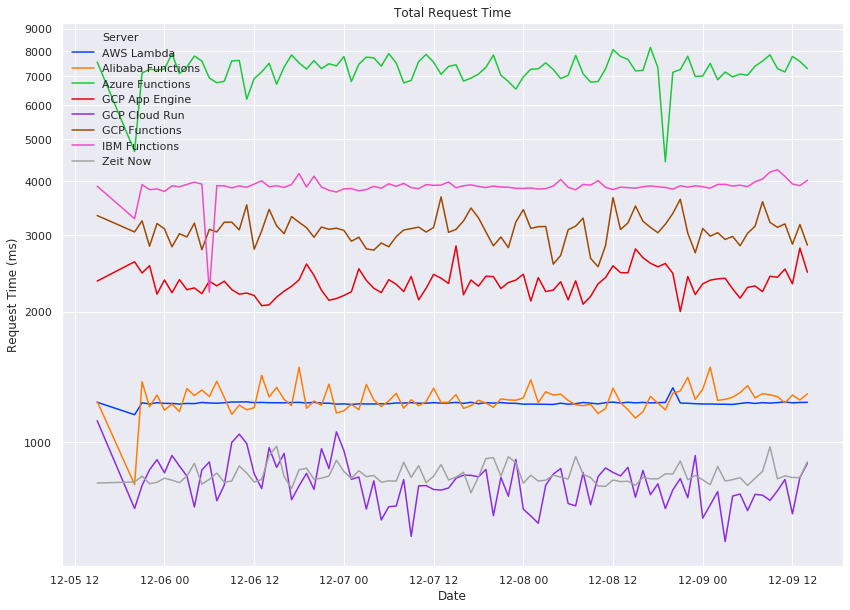
\includegraphics[width=14cm]{perfovertime.png}
\centering
\caption{Performance over time of all services tested.}
\label{Fig:performance}
\end{figure}


\subsection{Compute performance}
In Figure \ref{Fig:cputime}
we see the cumulative frequencies for the image processing time
as measured by the server, split by concurrency level (single and multi test phase) and cold/warm starts.


\begin{figure}[h]
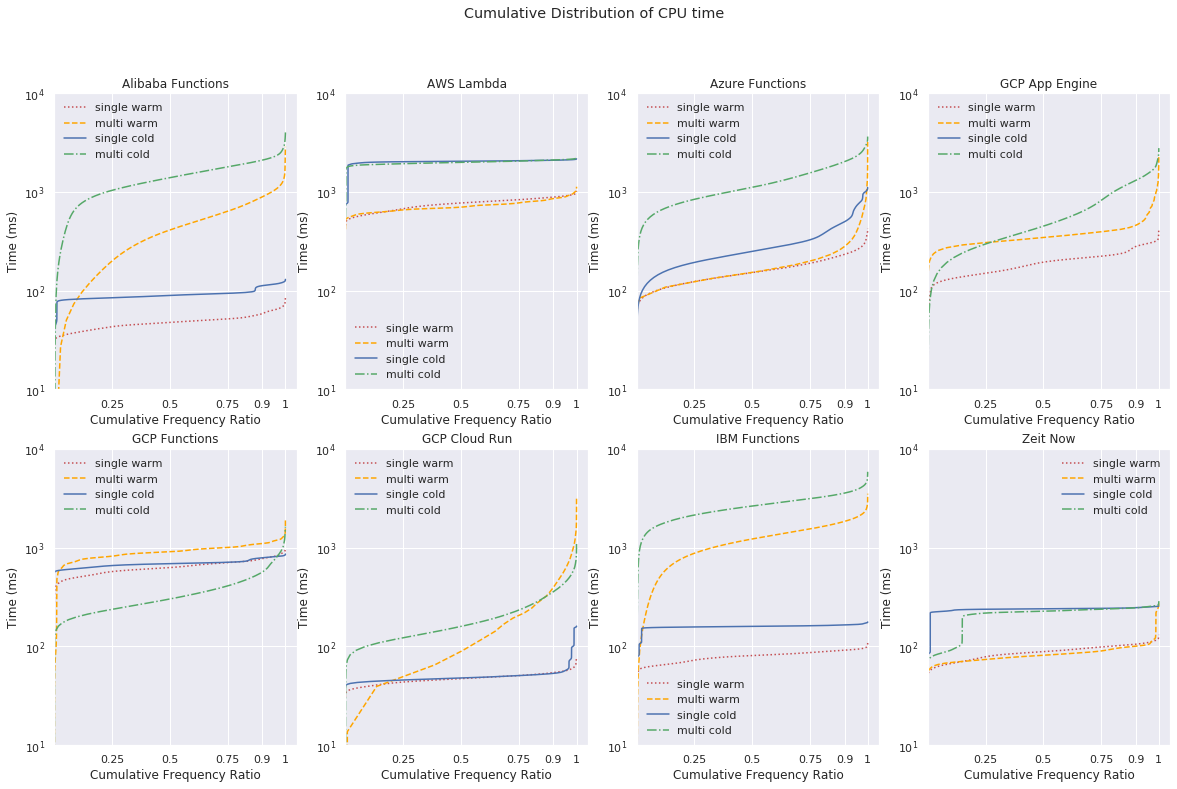
\includegraphics[width=14cm]{cputime.png}
\centering
\caption{Acumulative distribution of CPU time.}
\label{Fig:cputime}
\end{figure}


\subsection{Overhead}

In Figure \ref{Fig:overhead}
we see the cumulative frequencies for the overhead time
(total roundtrip time - server processing time) % todo: maths
split by concurrency level and cold/warm starts.
With all else being equal,
we atrribute the difference to time spent conducting a cold start.

% todo figure 3:
% explain single v multi in legend



\begin{figure}[h]
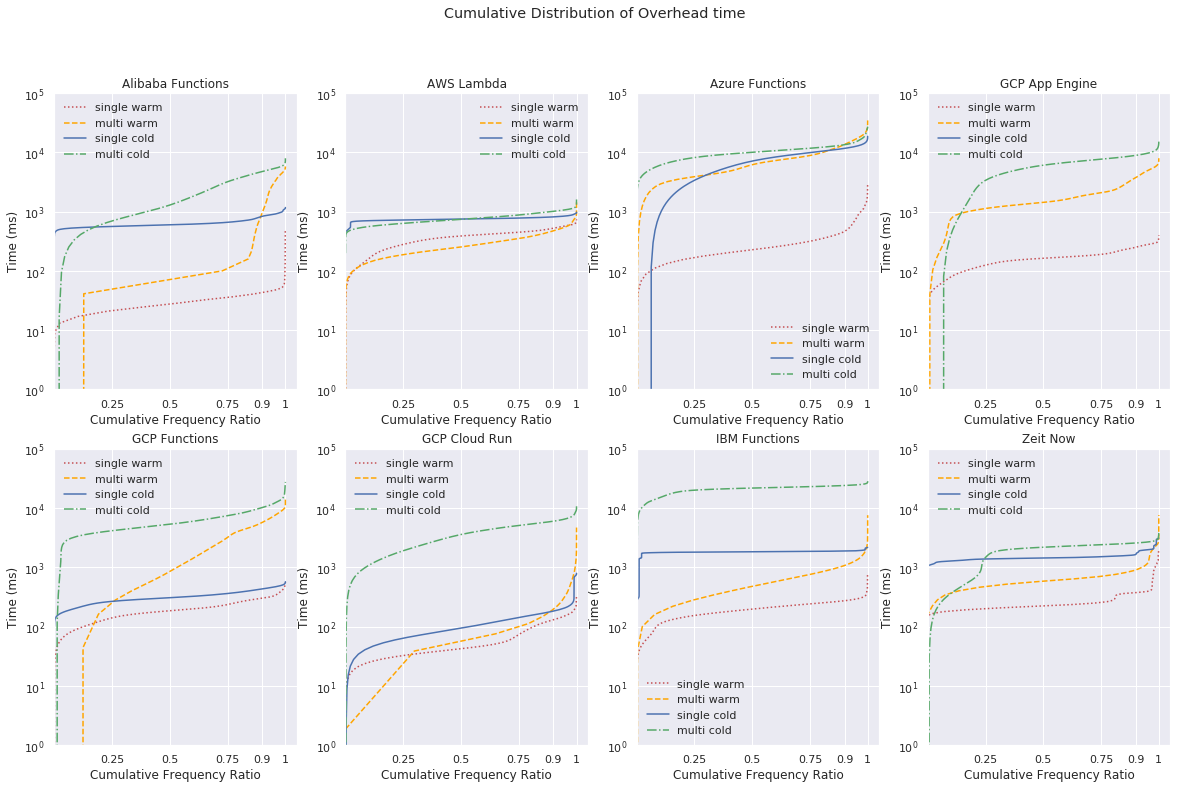
\includegraphics[width=14cm]{overhead.png}
\centering
\caption{Acumulative distribution of overhead time.}
\label{Fig:overhead}
\end{figure}



\section{Discussion}
\label{discussion}

\subsection{Scaling}
From Table \ref{Tab:multi}
we observed elevated failure rates for Alibaba Function Compute.
Their documentation \cite{ali}
states they have a limit of 50 instances per service,
and even though our client places a strict limit of 50 inflight requests at any point in time,
their scheduler might not be keeping up
in either reusing an instance or cleaning it up before the next request arrives.

Also from Table \ref{Tab:multi}
we can see the average number of unique instances per test cycle.
Ideally, this number would be 50,
to match the number of parallel requests we are sending.

On the low end,
Azure Functions is notable for only starting 4 instances.
This may be from a documented limitation \cite{azure}
of only starting at most 1 instance per second with HTTP triggers.
Their load balancers still hold the requests in queue,
but they appear to be reluctant to start new instances even as sufficient time has passed.

At the high end,
we configured GCP Cloud Run to accept up to 5 concurrent requests per instance,
expecting it to utilise the available memory and CPU more efficiently as this was one of its main selling points.
However, their scheduler also took CPU utilitzation into account,
limiting the usefulness of setting a higher concurrency level with our CPU intensive task.
In hindsight, setting the concurrency level to 1 would have been a fairer comparison.

From Figure \ref{Fig:cputime} we can see for AWS, Azure, Zeit, and GCP Functions,
we saw good isolation of workloads,
they performed similarly for warm requests at both concurrency levels.
GCP Cloud Run saw an expected degradation in performance from handling multiple requests,
While Alibaba and IBM were serverely impacted.




\subsection{Warm vs Cold Starts}
An often cited concern of using truly on-demand compute services is the cold start,
when the platforms have to start up a new instance to handle increases in load.
This is such a concern that some some platforms have specific features
built to keep your instances warm, such as AWS Provisioned Concurrency \cite{ams}
and Azure Functions Premium Plan.

Our results in Figure \ref{Fig:overhead}
show that, as expected, in most cases,
single concurrency cold starts are slower than warm starts
and the start times are highly consistent.
Cold start times are much more variable at higher concurrency levels,
with the exception of AWS Lambda which appears unaffected.
We suspect this could be due to having the system image on disk,
which is reusable as long as instances are on the same machine,
vs needing to retrieve the image over a network,
but we don't have a solid way of testing this.

What is unexpected is in Figure \ref{Fig:cputime},
that that cold starts affect CPU performance.
These instances consistently perform worse on a cold start,
even as they are reused for future requests.
Further testing would be needed to identify the root cause of this.

\subsection{Technologies}
GCP App Engine is the oldest technology being compared.
Under the hood it appears to be an NGINX reverse proxying Python apps through Gunicorn.
Its scaling is controlled by CPU utilization,
and in our case a heavy workload pushes that up
and limits the concurrent requests a single instance can handle.
While it can scale to zero instances,
each instance has a high (15 minute) startup fee \cite{gcp}
resulting in higher costs for short spikes in traffic.

The current generation of FaaS are built on a wide variety of technologies.
AWS and GCP have publicly stated that they use their own VMs,
Firecracker and gVisor respectively, to isolate workloads.
The results from Figure \ref{Fig:overhead}
show they provide a highly consistent environment even under load.
Zeit Now uses AWS datacenters \cite{zn}
for their serverless offering.
They behave similarly to AWS Lambda
and we believe that is what they use, but with the largest machine type.
Alibaba Functions, Azure Functions, and IBM Functions
all appear to be implemented on containers,
as either their developer tooling or documentation
hint at the possiblitily of customizing the runtime in not very well documentated ways.
Both Alibaba and IBM exhibit similar characteristics of degraded performance under load,
possibliy from poor isolation between workloads.

GCP Cloud Run is a fully managed container runtime implementing the Kubernetes Serving API,
and the only service we tested that exposed the Docker runtime directly.
As expected, single concurrency performance is consistent
but drops when more requests are routed to a single instance.
As the industry moves to converge on Kubernetes as a common interface and runtime,
we expect more fully integrated products in this space in the future.
While other platforms provide container runtimes or hosted Kubernetes,
they are at a lower level in the stack and don't provide the full functionality we were looking for.




\section{Conclusion}

% todo write conclusion

% AWS lambda for stability
% others might work if workload wasn't cpu bound



\bibliography{references}
\bibliographystyle{unsrt}


%Questions for sean:
%For some reason I cannot open sci hub in spain. Could you open this link (https://sci-hub.se/10.1002/cpe.4792) and send me a screenshoot or the titel of the paper? I will get it from uva lib.
%Secction introducction: FaaS, CaaS, etc. Aren't the current definitins good enought?
%Section results, overhead your comment % todo: maths. What do you mean?
%Which is the colorful paper?, narrow description pls.
%Methods section: It is necessary to mention web framework in the table 1 if its not mentioned in the text?


\end{document}
